% To generate 16:9 slides, use the following line:
% \documentclass[10pt, compress, aspectratio=169]{beamer}

\documentclass[10pt, compress]{beamer}

\usetheme[numbering=fraction, progressbar=none, titleformat=smallcaps, sectionpage=none]{metropolis}

\usepackage{sourcecodepro}
\usepackage{booktabs}
\usepackage{array}
\usepackage{listings}
\usepackage{graphicx}
\usepackage[english]{babel}
\usepackage[scale=2]{ccicons}
\usepackage{url}
\usepackage{relsize}
\usepackage{wasysym}
\usepackage{caption}

\usepackage{pgfplots}
\usepgfplotslibrary{dateplot}

\definecolor{Base}{HTML}{191F26}
\definecolor{Accent}{HTML}{157FFF}

\setbeamercolor{alerted text}{fg=Accent}
\setbeamercolor{frametitle}{bg=Base}

\setsansfont[BoldFont={Source Sans Pro Semibold},
              Numbers={OldStyle}]{Source Sans Pro}

\lstset{ %
  backgroundcolor={},
  basicstyle=\ttfamily\footnotesize,
  breakatwhitespace=true,
  breaklines=true,
  captionpos=n,
  commentstyle=\color{Accent},
  escapeinside={\%*}{*)},
  extendedchars=true,
  frame=n,
  keywordstyle=\color{Accent},
  language=C++,
  rulecolor=\color{black},
  showspaces=false,
  showstringspaces=false,
  showtabs=false,
  stepnumber=2,
  stringstyle=\color{gray},
  tabsize=2,
  keywords={thrust,plus,device_vector, copy,transform,begin,end, copyin,
  copyout, acc, \_\_global\_\_, void, int, float, main, threadIdx, blockIdx,
  blockDim, if, else, malloc, NULL, cudaMalloc, cudaMemcpy, cudaSuccess,
  cudaGetLastError, cudaDeviceSynchronize, cudaFree, cudaMemcpyDeviceToHost,
  cudaMemcpyHostToDevice, const, data, independent, kernels, loop,
  fprintf, stderr, cudaGetErrorString, EXIT_FAILURE, for, dim3},
  otherkeywords={::, \#pragma, \#include, <<<,>>>, \&, \*, +, -, /, [, ], >, <}
}

\renewcommand*{\UrlFont}{\ttfamily\smaller\relax}

\graphicspath{{../img/}}

\title{3D Real-time Indoor Localization via Broadband Nonlinear Backscatter}
\author{\footnotesize Lucas Morais \\ {\scriptsize \emph{morais.lucas.h@gmail.com}} \\
\footnotesize Lucas Kanashiro \\ {\scriptsize \emph{lkd@ime.usp.br}} \\
\footnotesize Pedro Bruel \\ {\scriptsize \emph{phrb@ime.usp.br}}}
\institute{
\includegraphics[height=2cm]{imelogo}\\[0.2cm] Instituto de Matemática e Estatística \\ Universidade de São Paulo}
\date{\scriptsize \today}

\begin{document}

\maketitle

\part{1}

\section*{Slides}
\begin{frame}
    \frametitle{Slides}
    \begin{center}
        
\includegraphics[width=.18\textwidth]{github}
    \end{center}
    Os \textit{slides} estão no \alert{GitHub}:

    \begin{itemize}
        \item \url{github.com/phrb/comp-movel-seminario}
    \end{itemize}
\end{frame}

\section*{Roteiro}
\begin{frame}
    \frametitle{Roteiro}
    \setbeamertemplate{section in toc}[sections numbered]
    \tableofcontents[hideallsubsections,part=1]
    \tableofcontents[hideallsubsections,part=2]
    \tableofcontents[hideallsubsections,part=3]
\end{frame}

\section{Introdução}


\begin{frame}
    \frametitle{Sobre o Artigo}
    \alert{Título:} 3D real-time indoor localization via broadband nonlinear backscatter in
    passive devices with centimeter precision

    \alert{Autores:} Yunfei Ma, Xiaonan Hui Edwin C. Kan, da \alert{Cornell University}

    \alert{Publicado em:} MobiCom '16 Proceedings of the 22nd Annual
    International Conference on Mobile Computing and Networking Pages 216-229

\end{frame}

\begin{frame}
  \frametitle{Contribuições Principais}

    Monitorar a posição de etiquetas RFID no espaço 3D:

    \begin{itemize}
      \item Com \alert{alta precisão} (erro de $3.5$cm)
      \item Em \alert{tempo real}: latência de $0.155$s
      \item Funciona em \alert{ambientes fechados e cheios de objetos}
      \item \alert{Não requer movimento relativo} ou \alert{nós de referência}
    \end{itemize}

    Hardware \& software co-design:

    \begin{itemize}
        \item \alert{Combinação de frequências}
        \item \alert{Modificações no algoritmo HMFCW} (heuristic optimized continuous wave ranging)
        \item Algoritmo de \alert{Localização 3D}
        \item \alert{Tag RFID não-linear}
    \end{itemize}
\end{frame}

\subsection{Aplicações}

\plain{Aplicações}

\begin{frame}
  \frametitle{Interação Humano-Máquina}
  \begin{itemize}
    \item  Controle/monitoração de braços robóticos
  \end{itemize}

  \begin{center}
    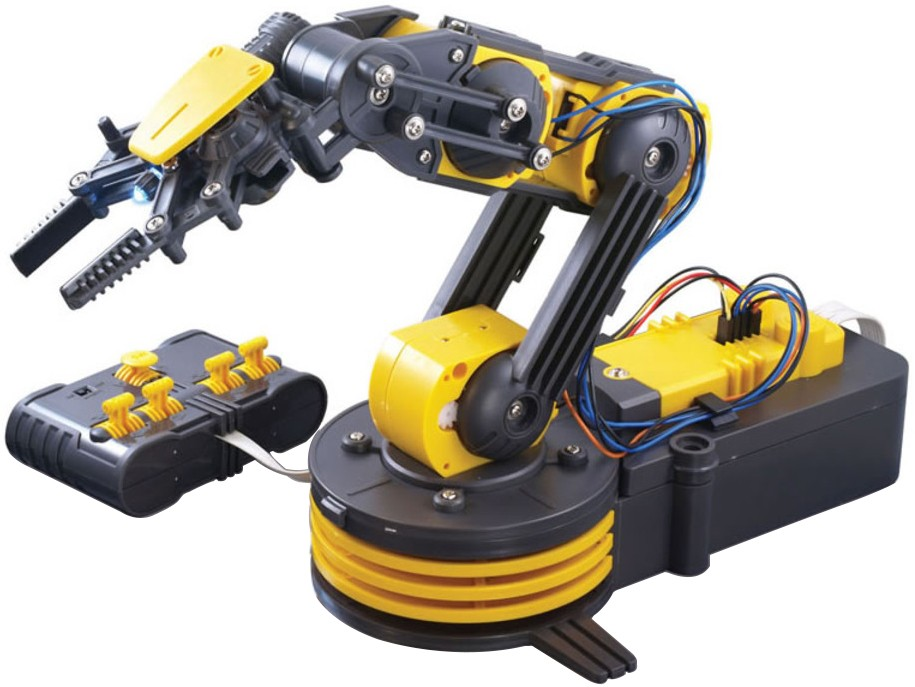
\includegraphics[width=.8\textwidth]{robot-arm}
  \end{center}
\end{frame}

\begin{frame}
  \frametitle{Interação Humano-Máquina}
  \begin{itemize}
    \item  Carros autônomos
  \end{itemize}

  \begin{center}
    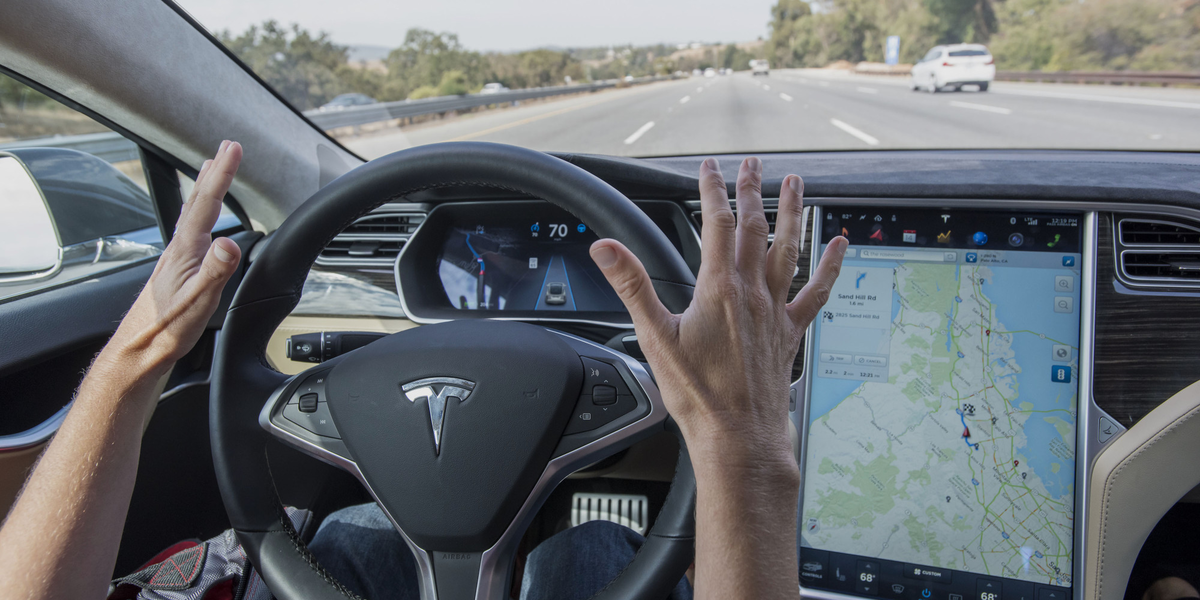
\includegraphics[width=\textwidth]{autopilot}
  \end{center}
\end{frame}

\begin{frame}
    \frametitle{Jogos \& Realidade aumentada}
    \begin{columns}[T,onlytextwidth]
        \column{.5\textwidth}
        \begin{center}
            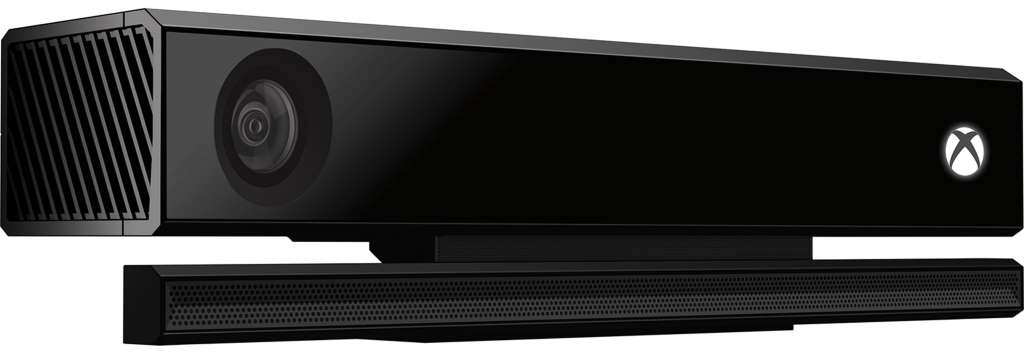
\includegraphics[width=.9\textwidth]{kinect-medium}
        \end{center}

        \column{.5\textwidth}
        \begin{center}
            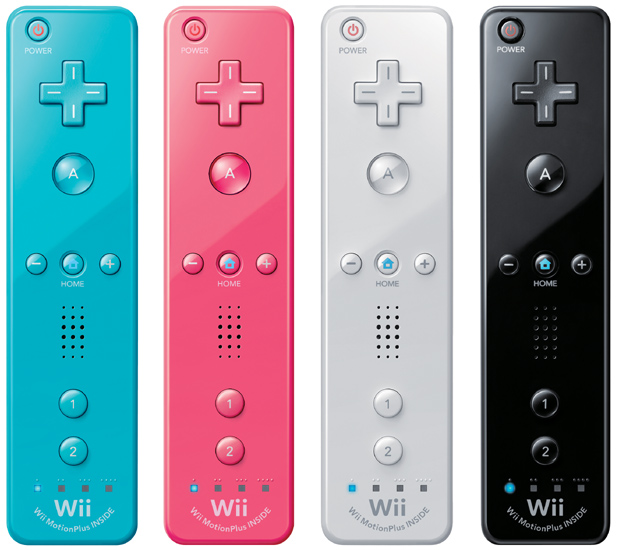
\includegraphics[width=0.5\textwidth]{wii-controller-more}
        \end{center}
    \end{columns}
\end{frame}

\begin{frame}
    \frametitle{Aplicações Comerciais}
        \begin{center}
            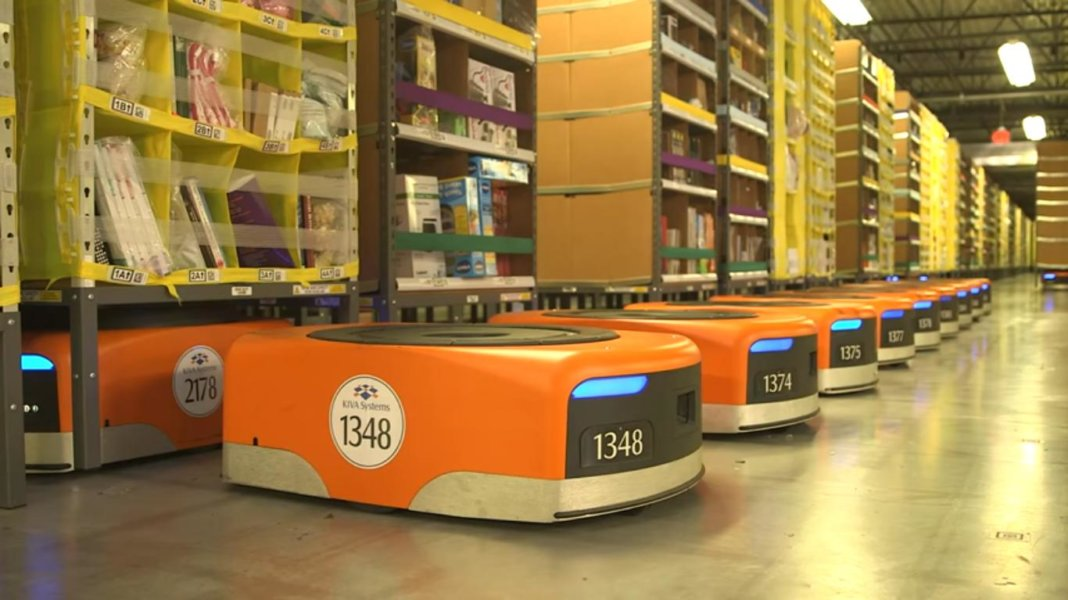
\includegraphics[width=.9\textwidth]{amazon-robots}
        \end{center}
\end{frame}

\begin{frame}
    \frametitle{Aplicações Comerciais}
        \begin{center}
            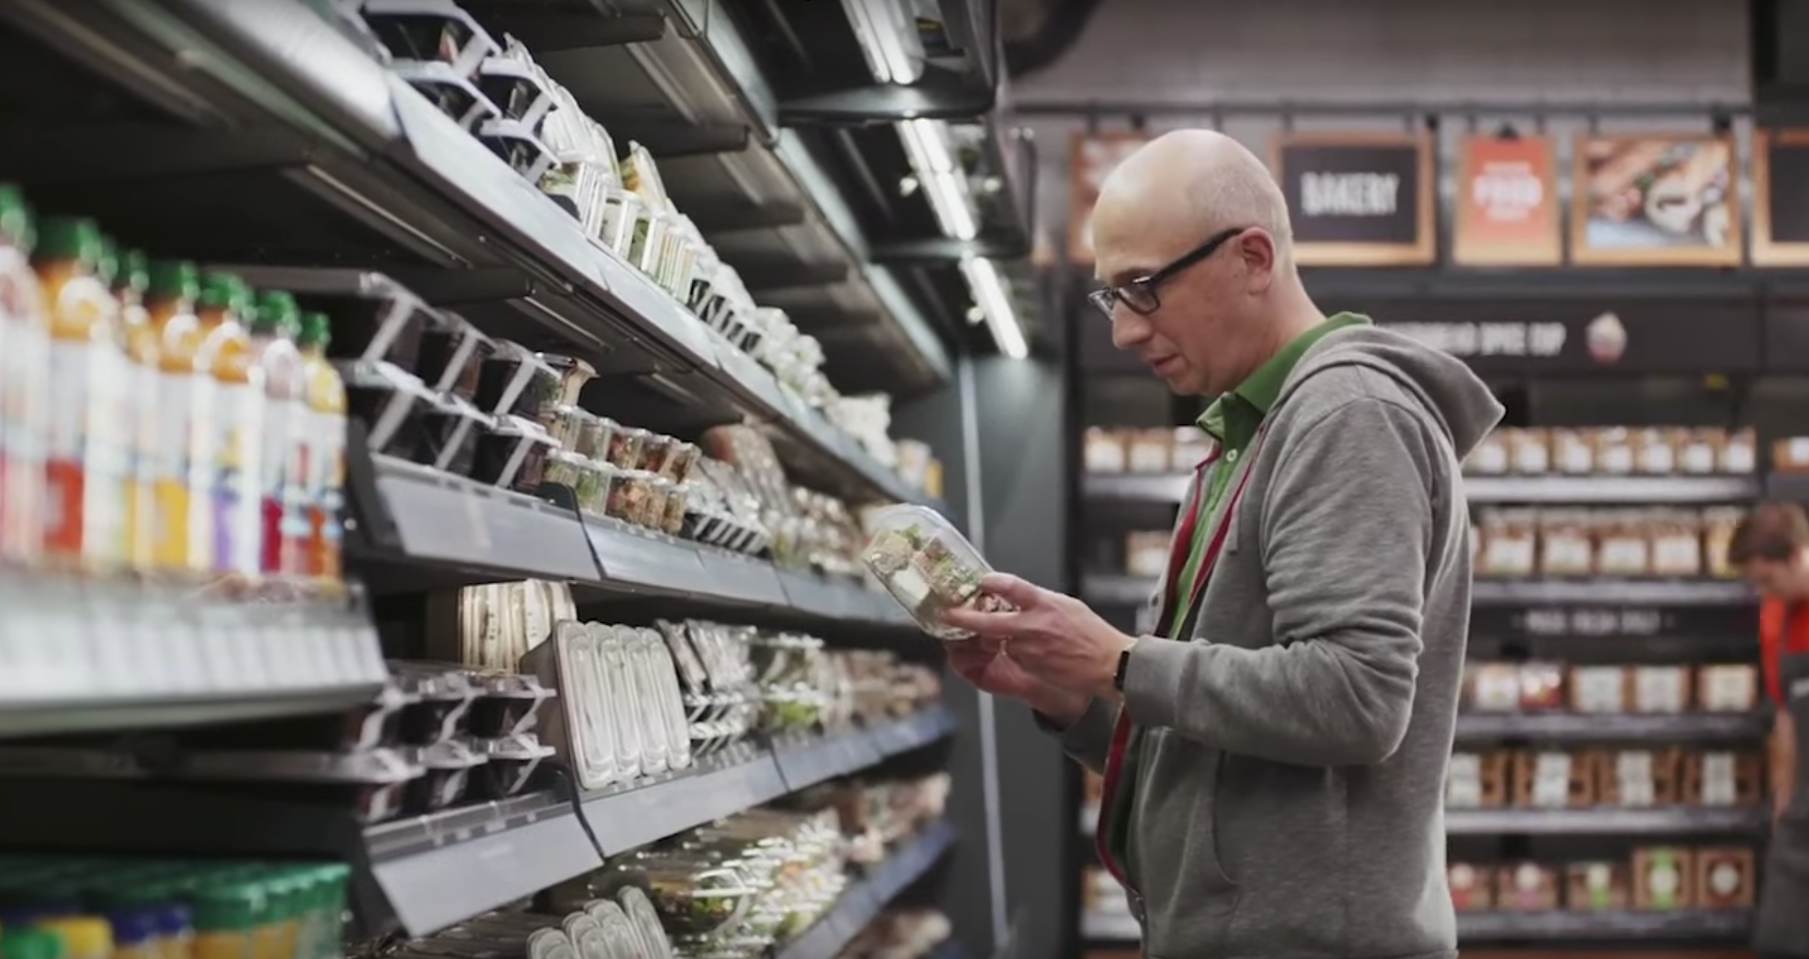
\includegraphics[width=.9\textwidth]{amazon-go-customer}
        \end{center}
\end{frame}

\begin{frame}
  \frametitle{3D-Tracking Hoje}

  Boa parte das técnicas de 3D-Tracking atuais são baseadas em visão
  computacional, com pequenas variações no:

  \begin{itemize}
    \item Aúmero de câmeras utilizadas
    \item Algoritmos de CV utilizados
    \item $\dots$
  \end{itemize}
\end{frame}

\begin{frame}
    \frametitle{Limitações Atuais}

    O problema já não está resolvido?

    \begin{itemize}
    \item  Alta complexidade computacional
    \item  Custo de implementação
    \item  Não funcionam em ambientes com obstáculos
    \end{itemize}

    \begin{center}
        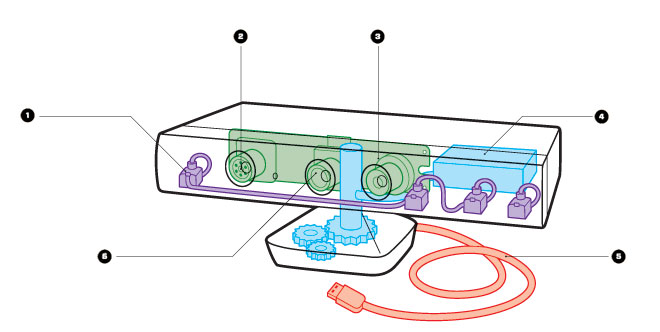
\includegraphics[width=0.8\textwidth]{kinect-diagram}
    \end{center}
\end{frame}


\begin{frame}
    \frametitle{3D-Tracking usando RFIDs}

    Vantagens:
    \begin{itemize}
    \item  \alert{Tags são muito baratas} ($0.1 \sim 0.2$ dólares)!
    \item  Técnica \alert{funciona mesmo com obstáculos}
    \item  \alert{Menor complexidade computacional}!
    \end{itemize}

    Problemas do estado-da-arte que a técnica do artigo supera:
    \begin{itemize}
    \item  Dependência de antenas de referência ou \emph{anchor nodes}
    \item  Dependência de conhecimento prévio da trajetória
    \item  Limitação a 2D-Tracking
    \end{itemize}
\end{frame}


\part{2}
\plain{Visão Geral}

\section{Visão Geral do Sistema}

\begin{frame}
    \frametitle{Visão Geral do Sistema}

    Quatro etapas principais:

    \begin{itemize}
        \item Obter \alert{informação sobre a fase}
        \item \alert{Detectar a fase} corretamente
        \item \alert{Variação de Frequências} (HMFCW)
        \item \alert{Cálculo da posição 3D}
    \end{itemize}
\end{frame}

\begin{frame}
    \frametitle{Visão Geral do Sistema}

    \begin{center}
        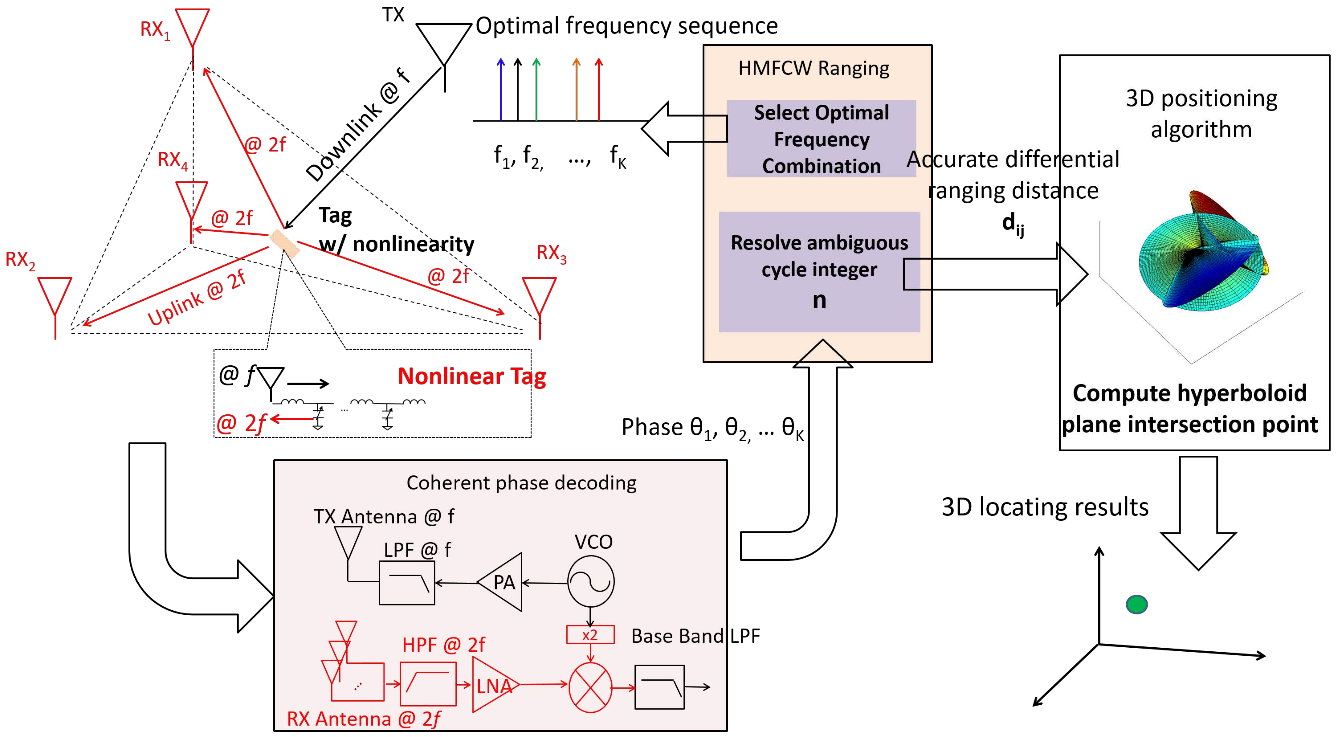
\includegraphics[width=1\textwidth]{overview}
    \end{center}
\end{frame}

\plain{Localização 3D}
\section{Soluções para Localização 3D}

\subsection{Eliminando o Auto-Bloqueio}

\begin{frame}
    \frametitle{Eliminando o Auto-Bloqueio}

    Entendendo o problema:
    \begin{itemize}
        \item Tags RFID consomem \alert{$\approx{}10\mu{}W$}
        \item Não têm energia para \alert{gerar sinais}
        \item Portanto, precisam \alert{refletir o sinal do emissor}
            \pause
        \item \alert{Como saber de onde vem uma reflexão?}
    \end{itemize}
\end{frame}

\begin{frame}
    \frametitle{Eliminando o Auto-Bloqueio}

    \begin{center}
        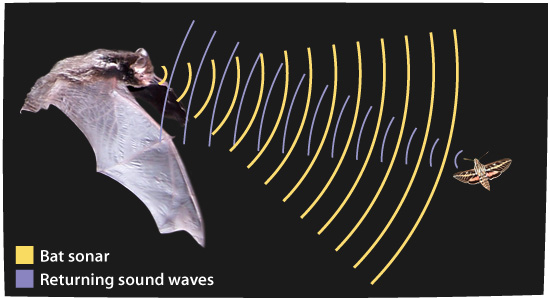
\includegraphics[width=.6\textwidth]{echolocation}
    \end{center}

    \pause
    \begin{columns}[T,onlytextwidth]
        \column{.25\textwidth}
        \begin{center}
            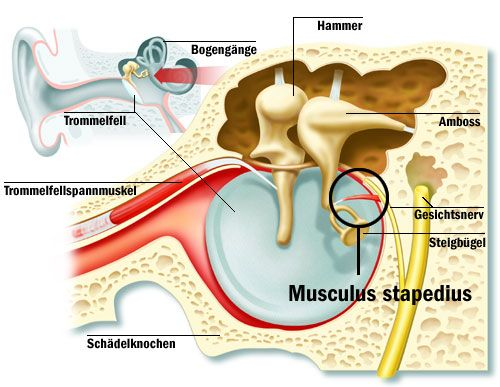
\includegraphics[width=\textwidth]{stapedius}
        \end{center}

        \pause

        \column{.25\textwidth}
        \begin{center}
            \vfill
            
\includegraphics[width=.8\textwidth]{mute}
        \end{center}

        \pause

        \column{.25\textwidth}
        \begin{center}
            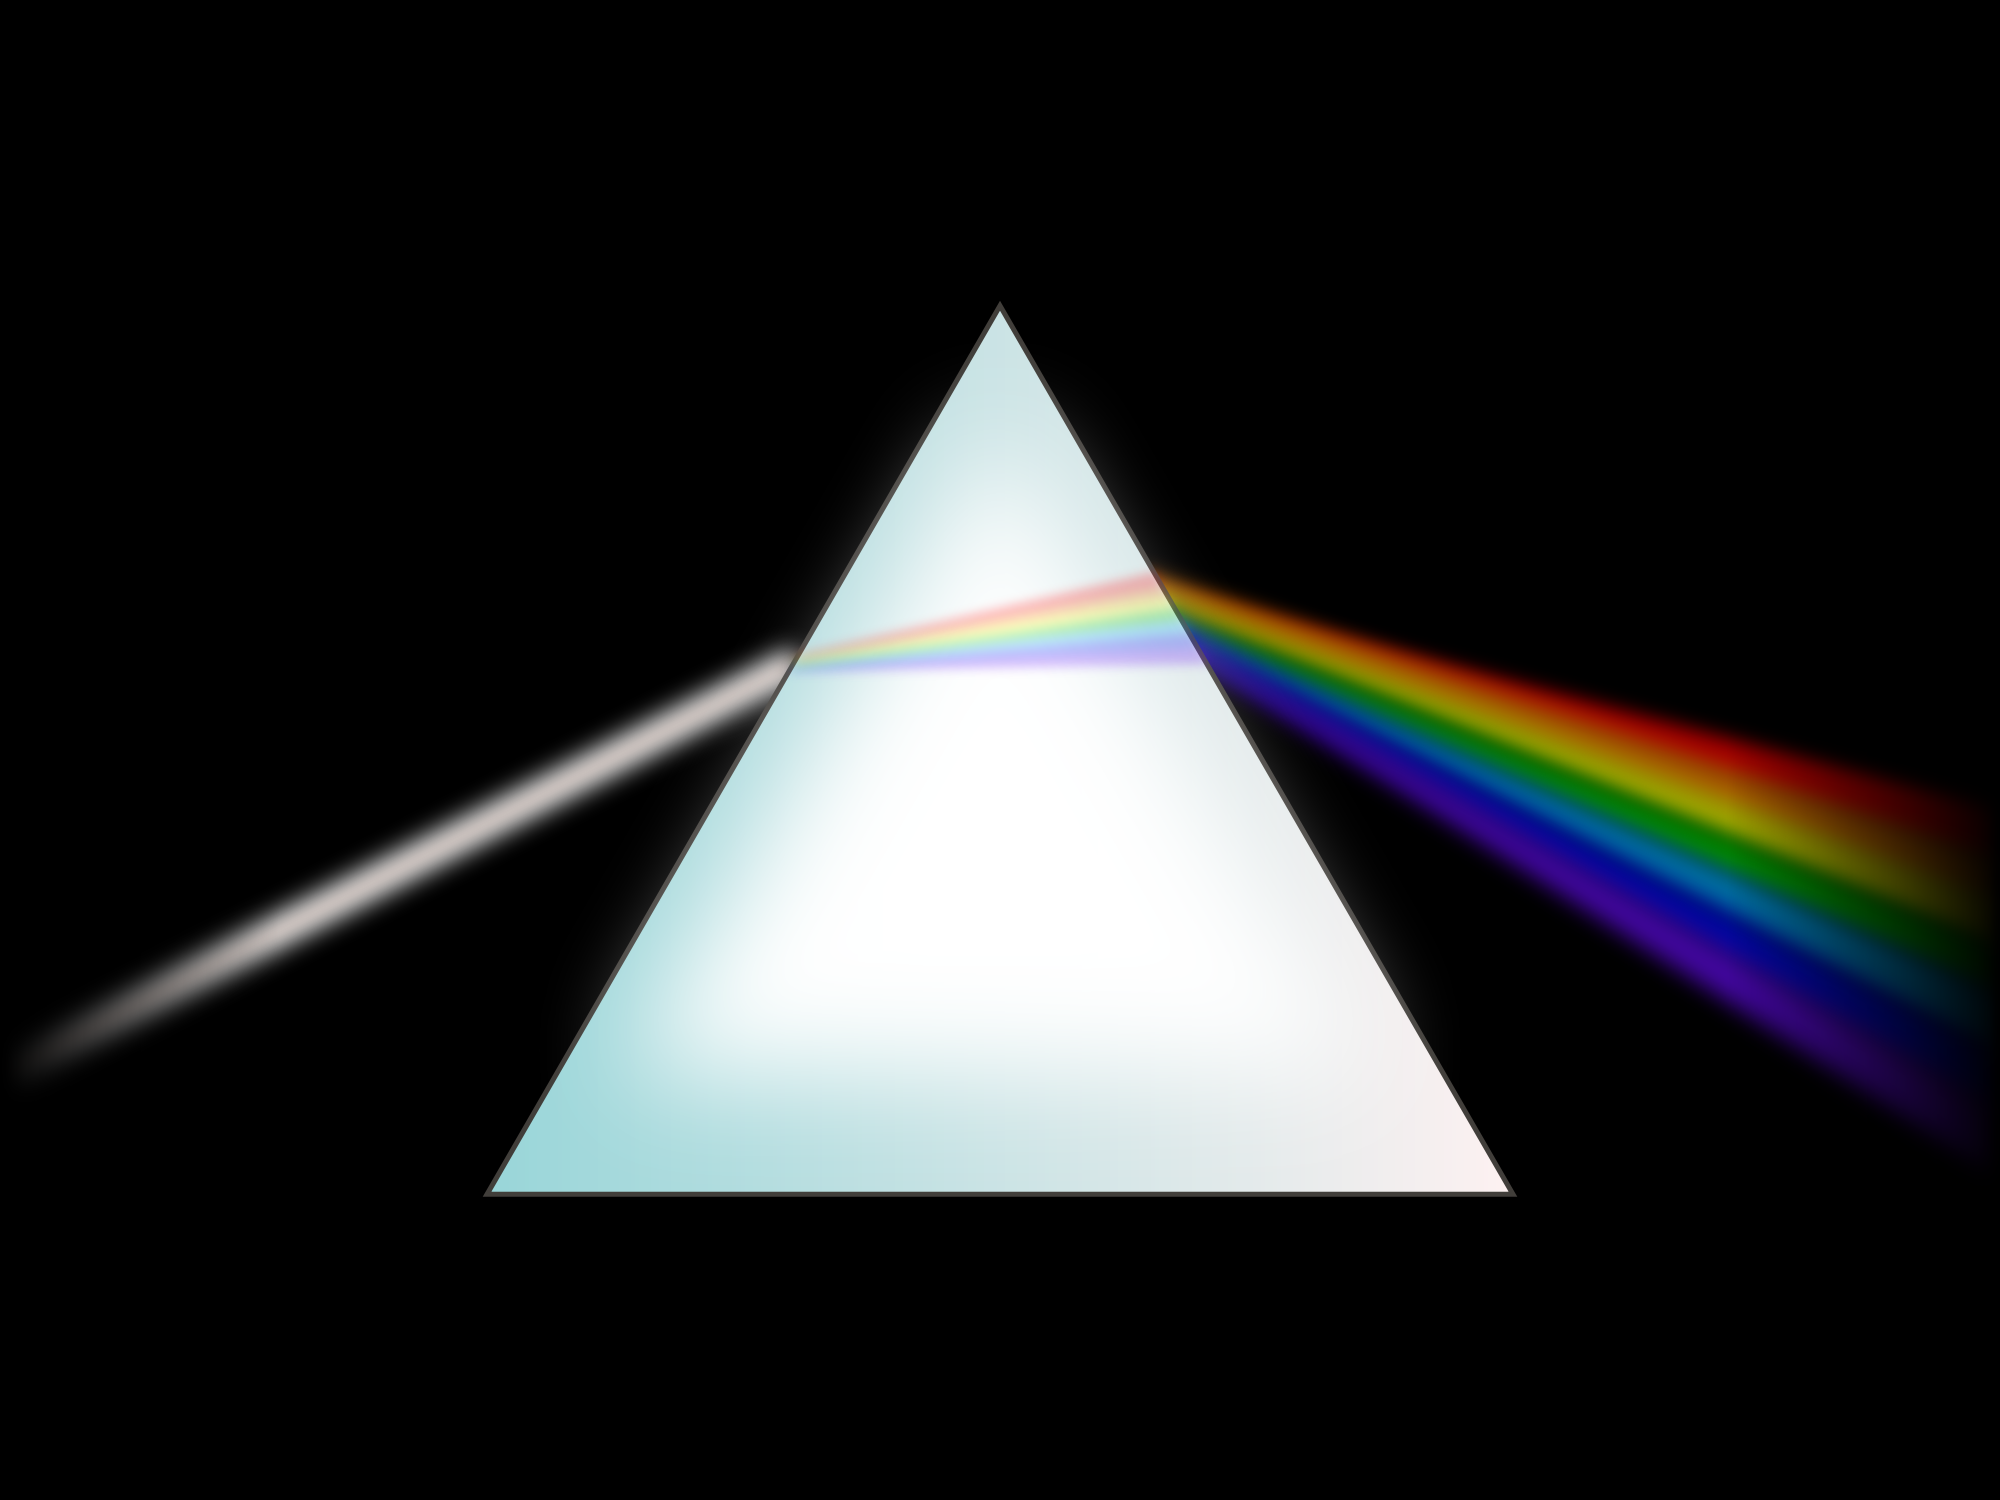
\includegraphics[width=1\textwidth]{spectrum}
        \end{center}

        \pause

        \column{.25\textwidth}
        \begin{center}
            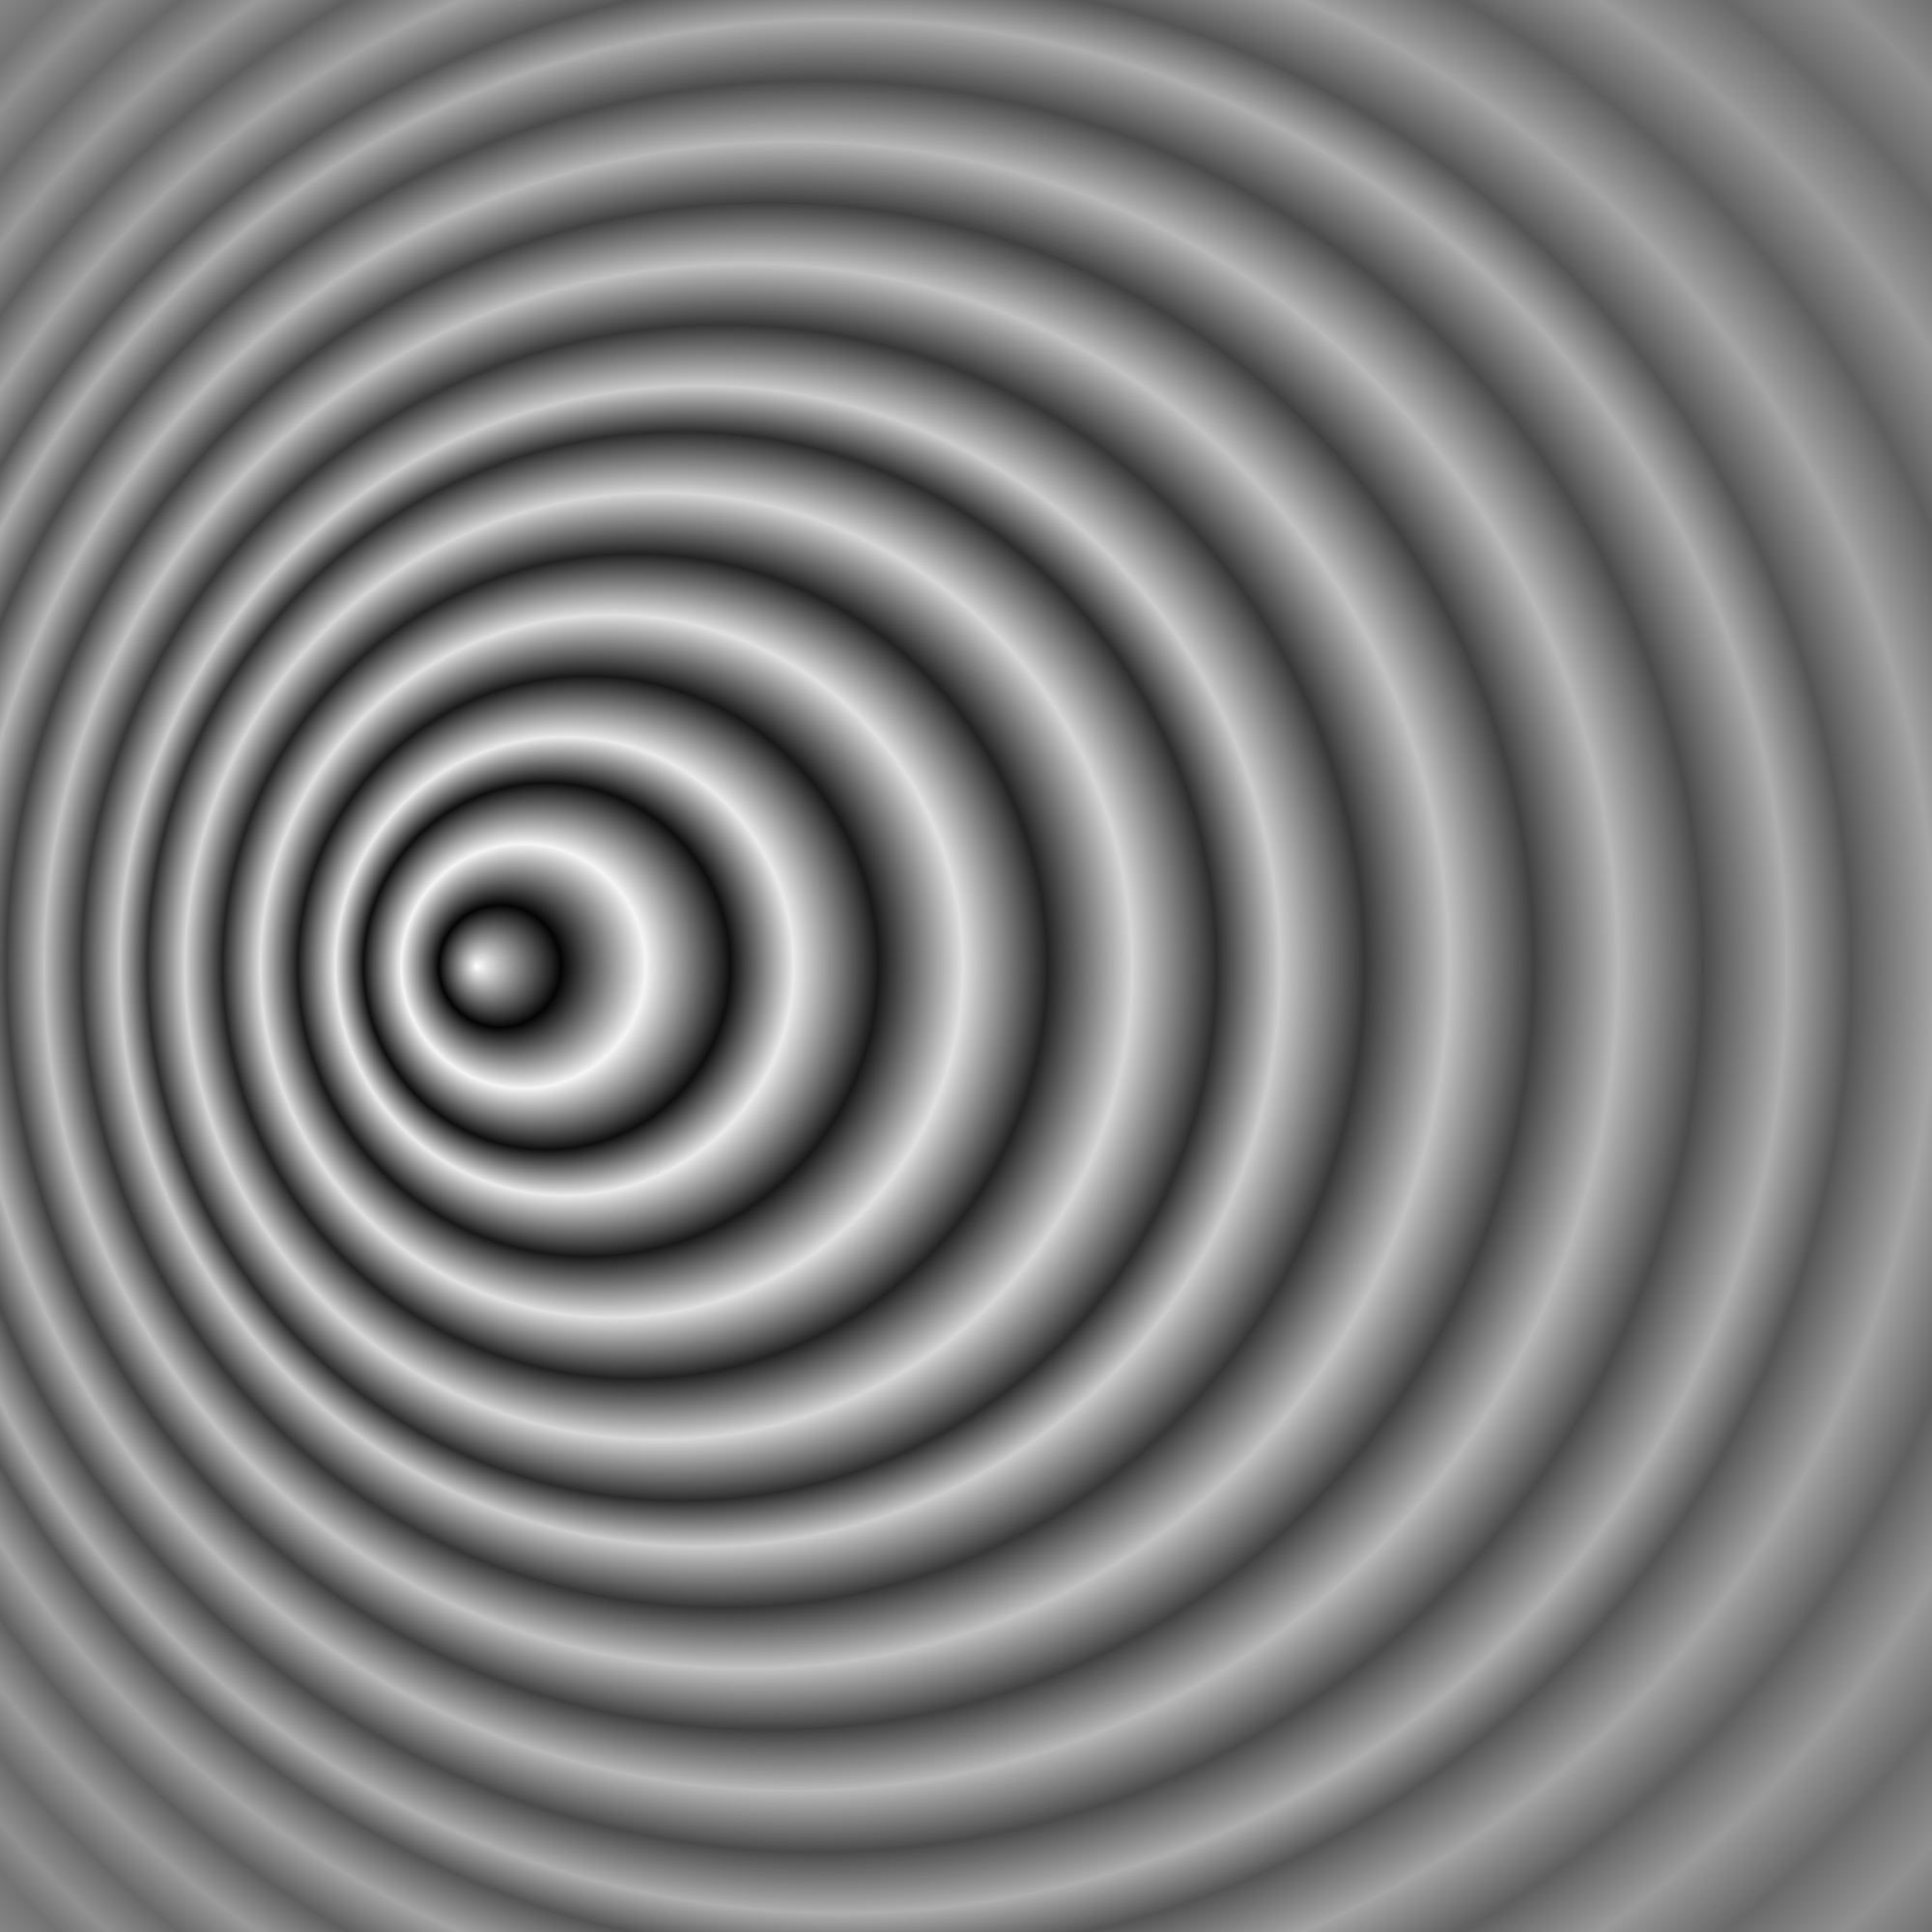
\includegraphics[width=.76\textwidth]{doppler}
        \end{center}
    \end{columns}
\end{frame}

\begin{frame}
    \frametitle{Eliminando o Auto-Bloqueio}

    Solução do artigo:
    \begin{itemize}
        \item Hardware e software \alert{co-design}
        \item Nova tag RFID: \alert{reflete harmônicos} do sinal recebido
        \item Algoritmo HMFCW: seleciona \alert{grupos de frequências}
    \end{itemize}

    \pause

    \begin{center}
        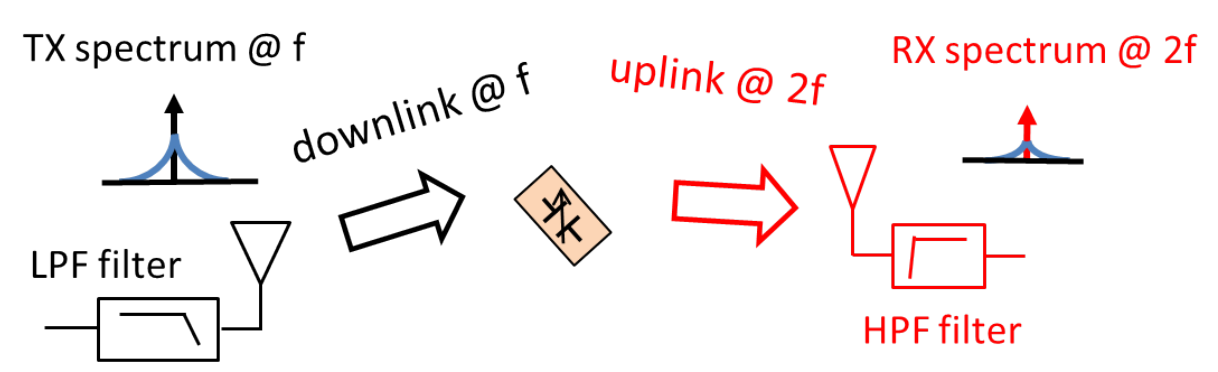
\includegraphics[width=.8\textwidth]{nonlinear-secondharmonic}
    \end{center}
\end{frame}

\subsection{Determinando a Variação de Frequências}
\begin{frame}
    \frametitle{Determinando a Variação de Frequências: Intuição}
    Problema:
    \begin{itemize}
        \item Como determinar corretamente a \alert{fase da reflexão}?
    \end{itemize}
    \begin{align*}
        d_{i}&,d_{j}: \; \text{distância da tag às antenas $i$ e $j$} \\
        \theta& \in [0, 2\pi)\\
        d_{ij} & = d_i - d_j \\
        d_{ij} & = \dfrac{\theta}{2\pi} \dfrac{\lambda}{2} + \alert{n} \dfrac{\lambda}{2}
    \end{align*}

    \pause

    \begin{center}
        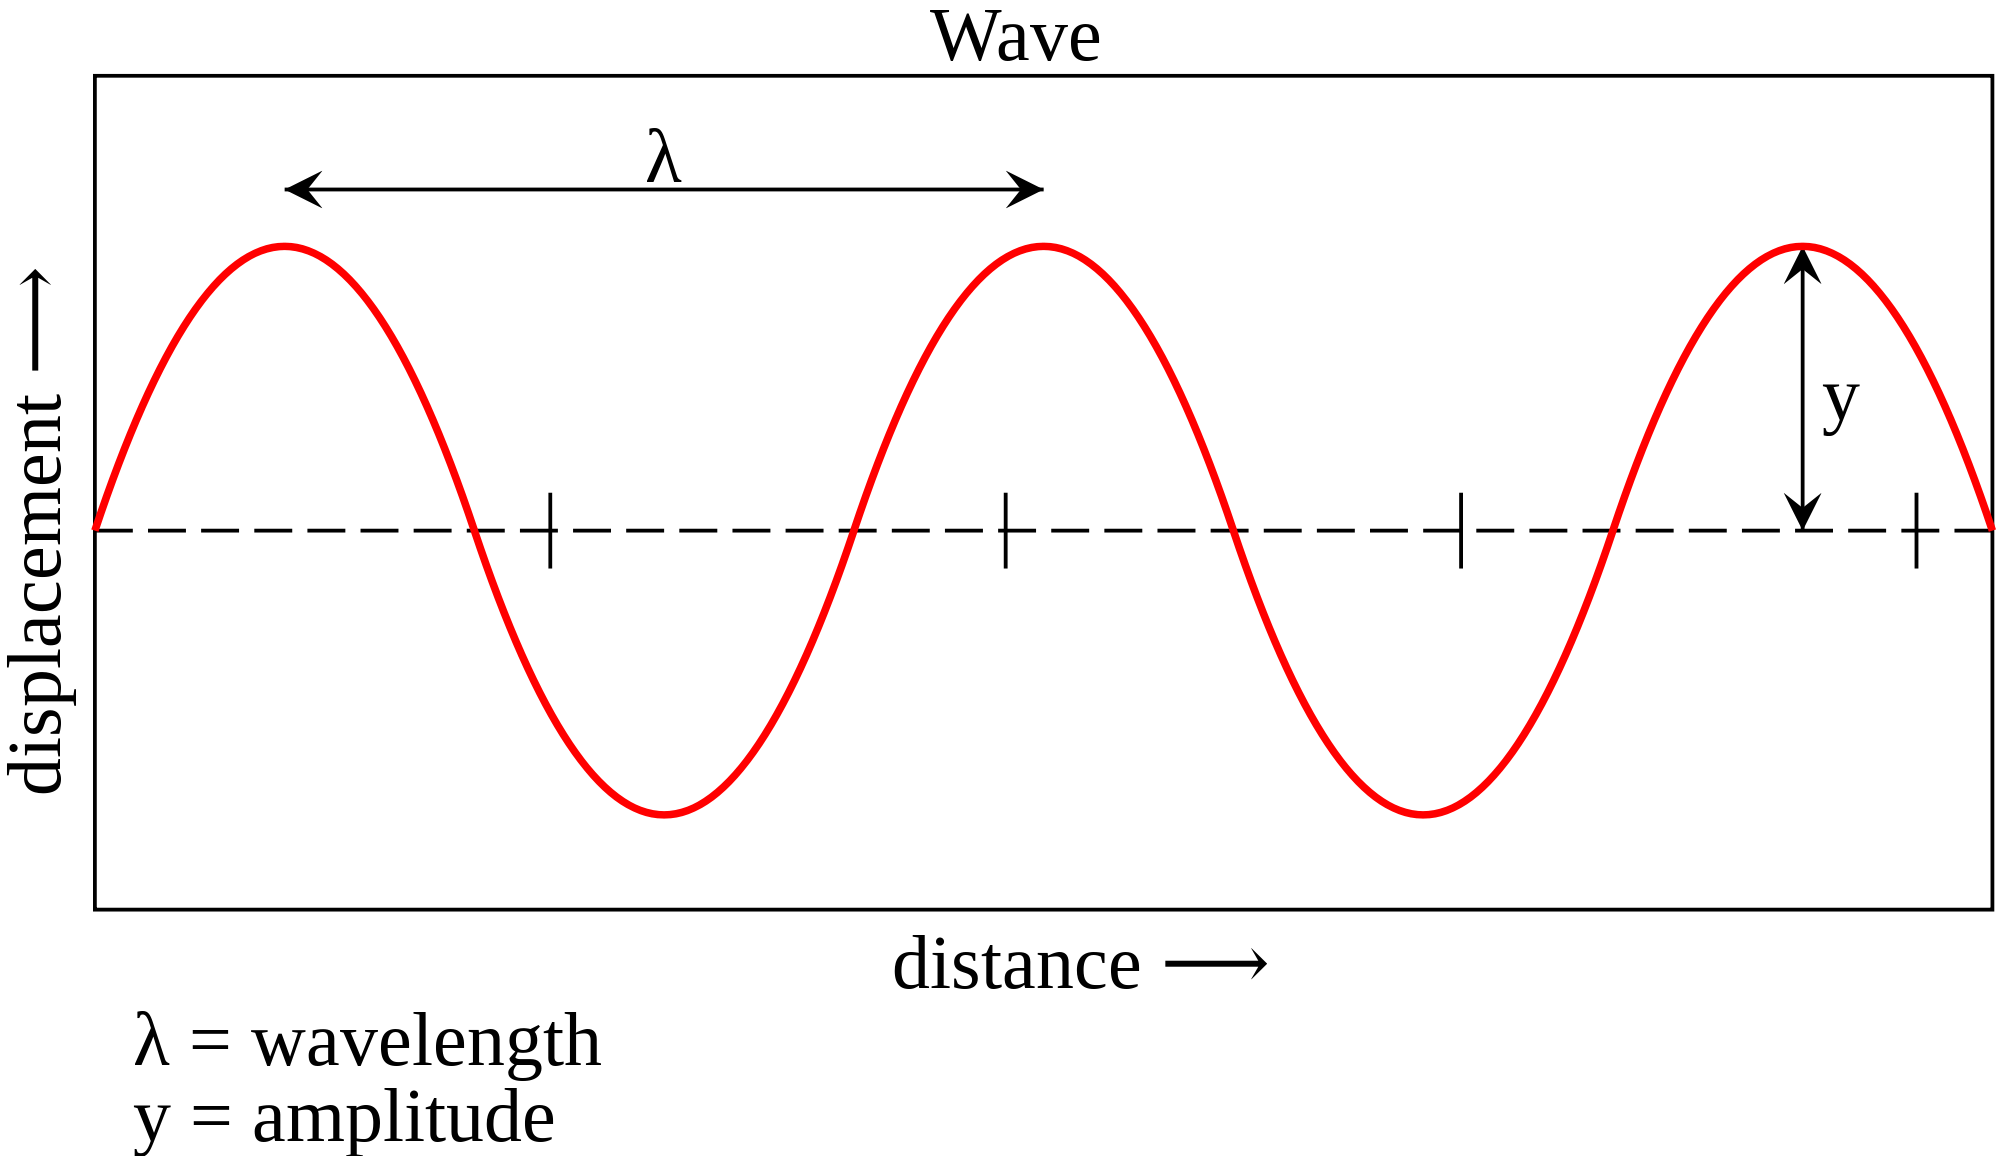
\includegraphics[width=.45\textwidth]{wave}
    \end{center}
\end{frame}

\begin{frame}
    \frametitle{Determinando a Variação de Frequências}

    Solução do artigo:
    \begin{itemize}
        \item \alert{Heuristic optimized continuous wave ranging} (HMFCW)
        \item \alert{Emitir simultaneamente um conjunto de frequências}
    \end{itemize}

    \pause

    \metroset{block=fill}
    \begin{block}{Provam que:}
        Usando uma \alert{combinação de frequências} é possível calcular $\alert{n}$ corretamente,
        desde que os \alert{erros de medição} e a \alert{distância} sejam \alert{limitados},
        e que a \alert{largura de banda seja grande o suficiente}.
    \end{block}
\end{frame}

\begin{frame}
    \frametitle{Determinando a Variação de Frequências}
    Como determinar a combinação de frequências?
    \begin{center}
        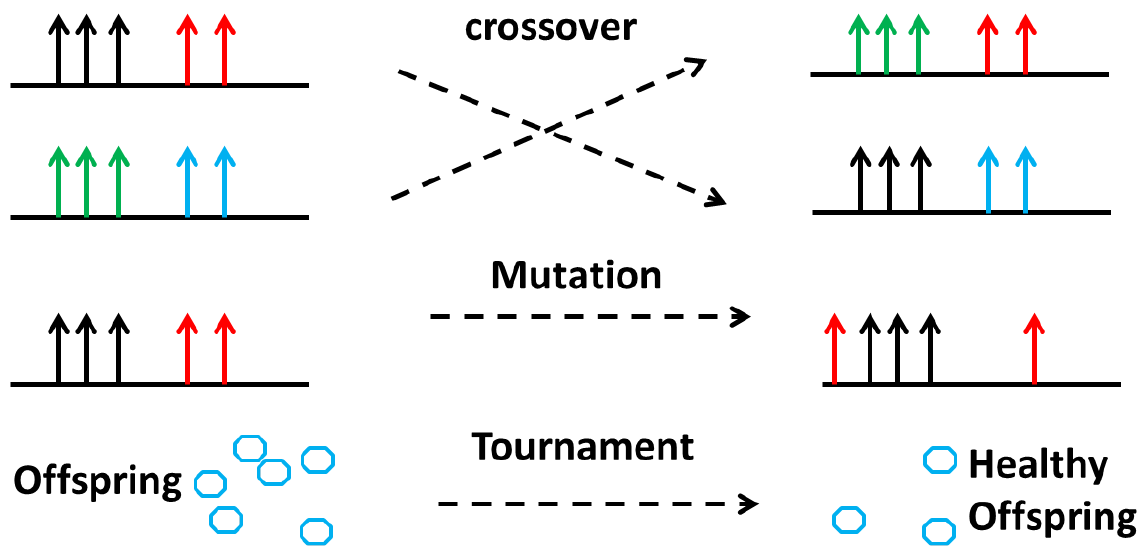
\includegraphics[width=.8\textwidth]{gas}
    \end{center}
\end{frame}

\subsection{Algoritmo de Localização 3D}
\begin{frame}
    \frametitle{Algoritmo de Localização 3D}
    Usando apenas \alert{duas antenas}:

    \begin{center}
        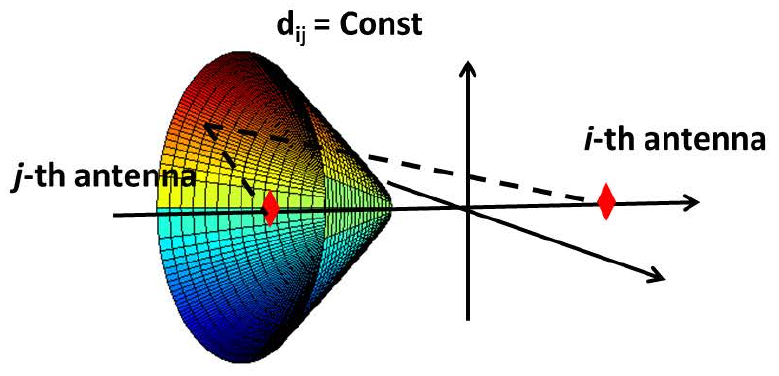
\includegraphics[width=.8\textwidth]{single-hyperboloid}
    \end{center}
\end{frame}

\begin{frame}
    \frametitle{Algoritmo de Localização 3D}
    \begin{center}
        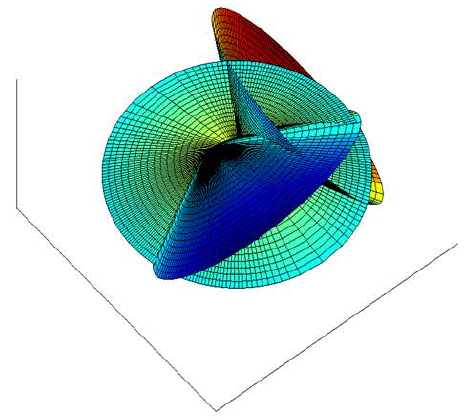
\includegraphics[width=.45\textwidth]{multiple-hyperboloids}
    \end{center}

    Como encontrar a \alert{intersecção dos hiperboloides}?
    \begin{itemize}
        \item Método \alert{Nonlinear Conjugate Gradient}
        \item Fórmula de \alert{Fletcher-Reeves}
        \item \alert{Geração aleatória do ponto inicial}
    \end{itemize}
\end{frame}


\part{3}
\section{Avaliação experimental}

\plain{Avaliação Experimental}

\subsection{Testbed}

\begin{frame}
  \frametitle{Testbed}

  \begin{figure}
          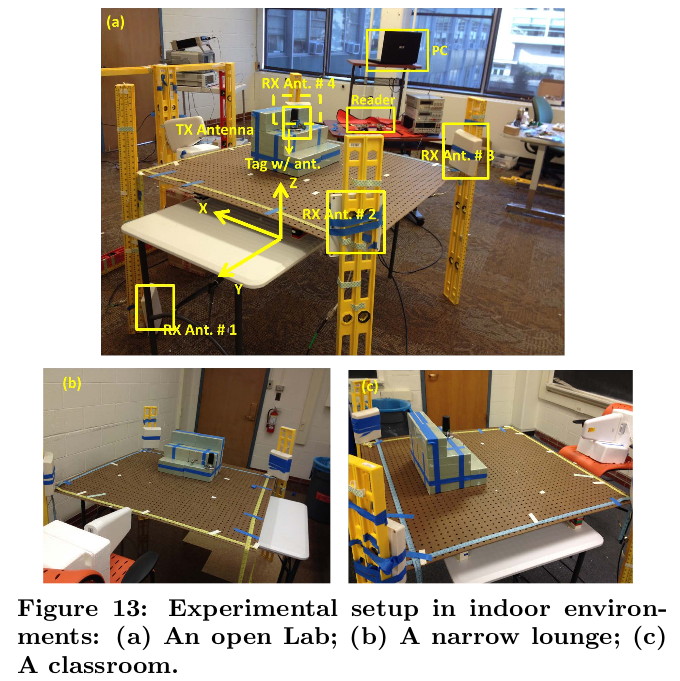
\includegraphics[scale=0.33]{testbed.png}
  \end{figure}
\end{frame}

\subsection{Experimentos}

\begin{frame}
  \frametitle{Medidas de Alcance 1D}

  \begin{figure}
          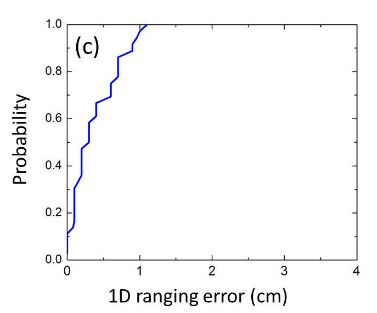
\includegraphics[width=6cm]{experiment_1D.png}
  \end{figure}
\end{frame}

\begin{frame}
  \frametitle{Medidas de Localização 2D}

  \begin{figure}
          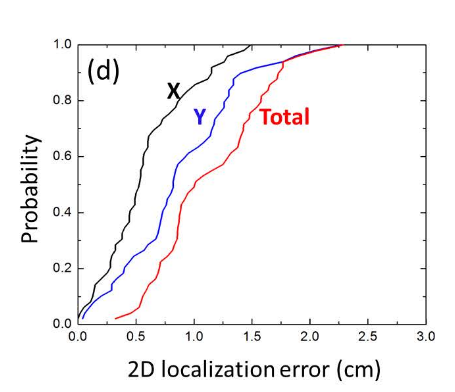
\includegraphics[width=5cm]{experiment_2D_probability.png}
          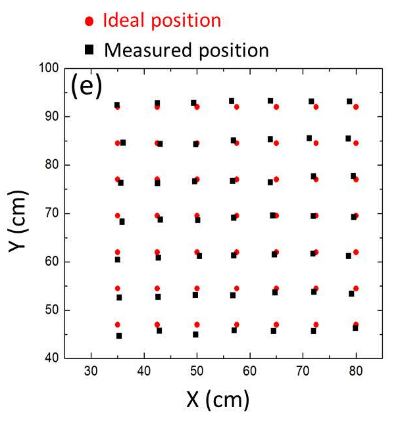
\includegraphics[width=5cm]{experiment_2D_position.png}
  \end{figure}
\end{frame}

\begin{frame}
  \frametitle{Medidas de Localização 3D}

  \begin{figure}
    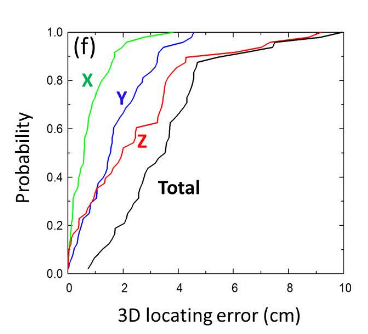
\includegraphics[width=4cm]{experiment_3D_in_open_lab.png}\hfil
    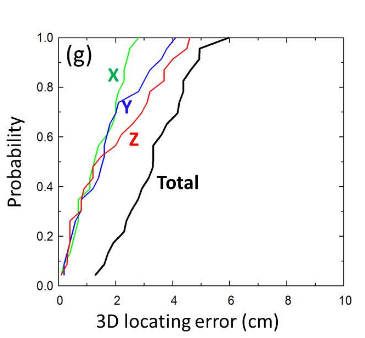
\includegraphics[width=4cm]{experiment_3D_in_narrow_lounge.png}\newline
    \hfil\hfil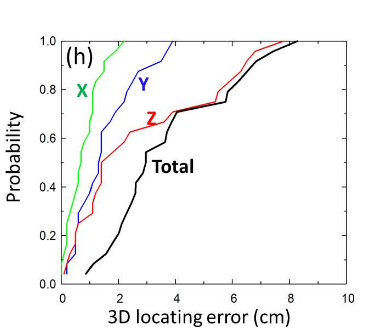
\includegraphics[width=4cm]{experiment_3D_in_classroom.png}
        \end{figure}
\end{frame}

\begin{frame}
  \frametitle{Localização com Elementos de Dispersão}

  \begin{figure}
          \centering
    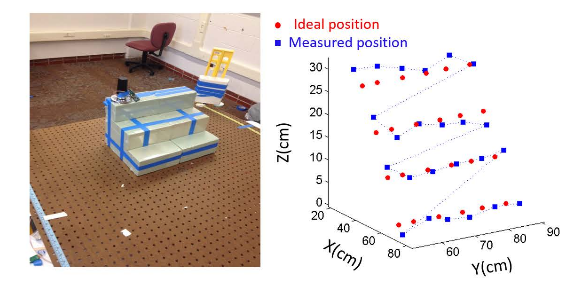
\includegraphics[width=7cm]{experiment_3D_without_scatter.png}
                \vfill
    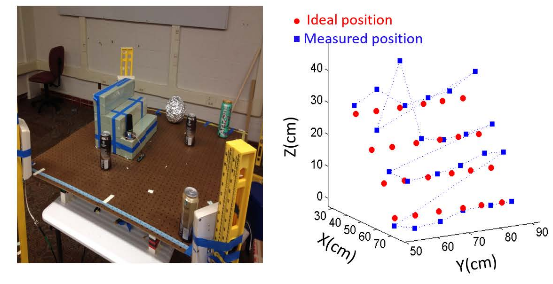
\includegraphics[width=7cm]{experiment_3D_with_5_scatters.png}
        \end{figure}
\end{frame}

\begin{frame}
  \frametitle{Localização com Elementos de Dispersão}

  \begin{figure}
          \vfill
          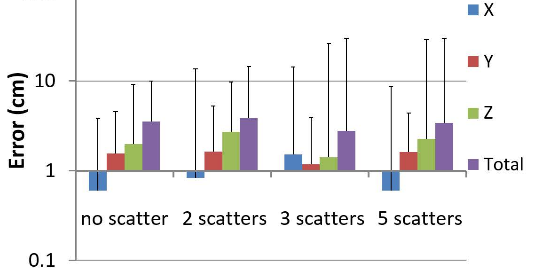
\includegraphics[width=9cm]{experiment_3D_error.png}
  \end{figure}
\end{frame}

\begin{frame}
  \frametitle{Monitoramento 3D em Tempo Real}

  \begin{figure}
          \vfill
          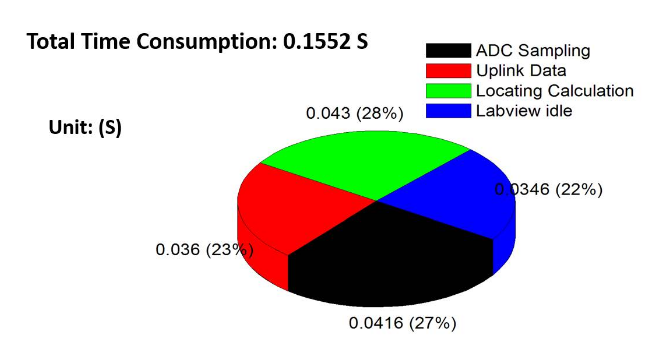
\includegraphics[width=9cm]{experiment_real_time_latency.png}
  \end{figure}
\end{frame}

\begin{frame}
  \frametitle{Vídeo de Apresentação}
    Vídeo de 1 minuto, no YouTube, sobre o artigo:
    \begin{itemize}
        \item \url{https://youtu.be/FwmQvAi7omo}
    \end{itemize}
\end{frame}

\section{Discussões}

\begin{frame}
  \frametitle{Discussões}

    \begin{itemize}
        \item Uso legítimo do espectro
            \begin{itemize}
                \item Legalidade na re-radiação harmônica
                \item Legalidade no emissor
            \end{itemize}
        \item Limitações no intervalo de leitura
        \item Custo da tecnologia
    \end{itemize}
\end{frame}

\subsection{Conclusão}

\begin{frame}
  \frametitle{Conclusão: Contribuições Principais}

    Monitorar a posição de etiquetas RFID no espaço 3D:

    \begin{itemize}
      \item Com \alert{alta precisão} (erro de $3.5$cm)
      \item Em \alert{tempo real}: latência de $0.155$s
      \item Funciona em \alert{ambientes fechados e cheios de objetos}
      \item \alert{Não requer movimento relativo} ou \alert{nós de referência}
    \end{itemize}

    Hardware \& software co-design:

    \begin{itemize}
        \item \alert{Combinação de frequências}
        \item \alert{Modificações no algoritmo HMFCW}
        \item Algoritmo de \alert{Localização 3D}
        \item \alert{Tag RFID não-linear}
    \end{itemize}
\end{frame}


\maketitle

\end{document}
